\section{Implementation, Integration and Test Plan}
The whole system presents the following components:
\begin{itemize}
    \item Application (myAPTracker): the application for iOS downloadable from the app store.
    \item Web Server.
    \item Application Server.
    \item Internal Database.
    \item External services such as authentication via social and notification managing.
\end{itemize}

Those elements have been implemented following a bottom up approach, in order to have an easier testing.
Our testing phase will mainly relies on UI testing, because most of the logic is on the back-end.
The main focus will be on the Application and on the Application server, because in the Application relies all the visual part and is the point from which the user can interact with the rest of the system; while the Application Server part contains all the relevant functions that make the Application works properly.\\
The following table presents the main functionalities of the system, highlighting for each of them the importance for the costumer and the difficulty of its implementation. 

\begin{table}[h!]
    \caption{Implementation and testing precedence}
    \label{tab:implementention_testing_precedences}
    \rowcolors{2}{gray!25}{white}
    \centering
    \begin{tabular}{c|c|c}
    \rowcolor{gray!50}
    \textbf{Functionality} & \textbf{Importance for customer} & \textbf{Difficulty}\\ \hline\hline
    Back-end & High & High\\
    Application views & High & High\\
    Local registration and Login & High & Low\\
    Social registration and Login & High & Medium\\
    Notification & Medium & High\\
    Scraper & High & Medium\\\hline
    \end{tabular}
\end{table}

All the functionalities described in this document relies on a DBMS that has to be implemented firstly.\\
According to table \ref{tab:implementention_testing_precedences} we decided to implement the functionalities following their importance.

\begin{itemize}
    \item \textbf{Back-end:} the back-end contains the fulcrum of all the system, since contains all the functions that are essential for the functioning of the system. The back-end is the communication point between the DB and the application and this connection is possible thanks to the use of multiple APIs.\\
    The testing details are not relevant for the purpose of this project.
    
    \item \textbf{Scraper:} this functionality is of relevant importance to populate the DB with Amazon products.\\
    To test this functionality we have taken different products (available or not on Amazon) and verified if the JSON that output the scraper was the correct one.
    
    \item \textbf{Application views:} the application views are the most important part of myAPTracker. The views have been realized for iPad and iPhone, with different designs according to the device dimensions.\\
    The testing of this part is crucial and it has been done with the XCTest framework of Swift. Different test has been done to see if elements were appearing on screen, to test the functionality of some views and also visual test regarding the redraw of the view based on some logic.

    \item \textbf{Local registration and Login:} the two functionalities are related to the local DB where the credential of a user are stored and then retrieved.\\
    In this parts is important to test the ability to save and retrieve User attributes from the DBMS correctly.
    
    \item \textbf{Social registration and Login:} the two functionalities are related to different external services, such as Google, Facebook and Apple (implemented using different methods).\\
    In this parts is important to test the ability to authenticate the user using the different external services.
    
    \item \textbf{Notification:} this functionality is implemented through Firebase and the use of the device table in the DB.\\
    To test the notification mechanism a test notification could be send to all the devices or to a precise device through Firebase.
\end{itemize}

\subsection{Testing}
We test both the logic and the User Interface of our application. Several tests have been done for all the typologies of supported device (iPhone, iPad and Apple Watch).
All the tests have a proper naming, defined by all the following items element separated by an \_:
\begin{itemize}
    \item test: all XCTest should start with the word test in order to be recognized as tests.
    \item Type of device: iPhone, iPad or Watch.
    \item Name of the view.
    \item Name of the UIElement or part of the view most involved in the current test.
    \item Action that the test is going to test.
\end{itemize}
For instance a proper name could be:\\ "test\_iPad\_SettingsView\_UserProfileInformation\_UserShowInfoAndGoBack".
For all the UITest the override of the "setUpWithError" function has been exploited to set up all the different tests in order to reach its correspondent view. This has been done in order to reduce as much as possible the duplication of code.
\\
Below are present the results of our tests, divided by type of tests.

\newpage
\subsubsection{Unit testing}
\begin{figure}[h!]
        \centering
        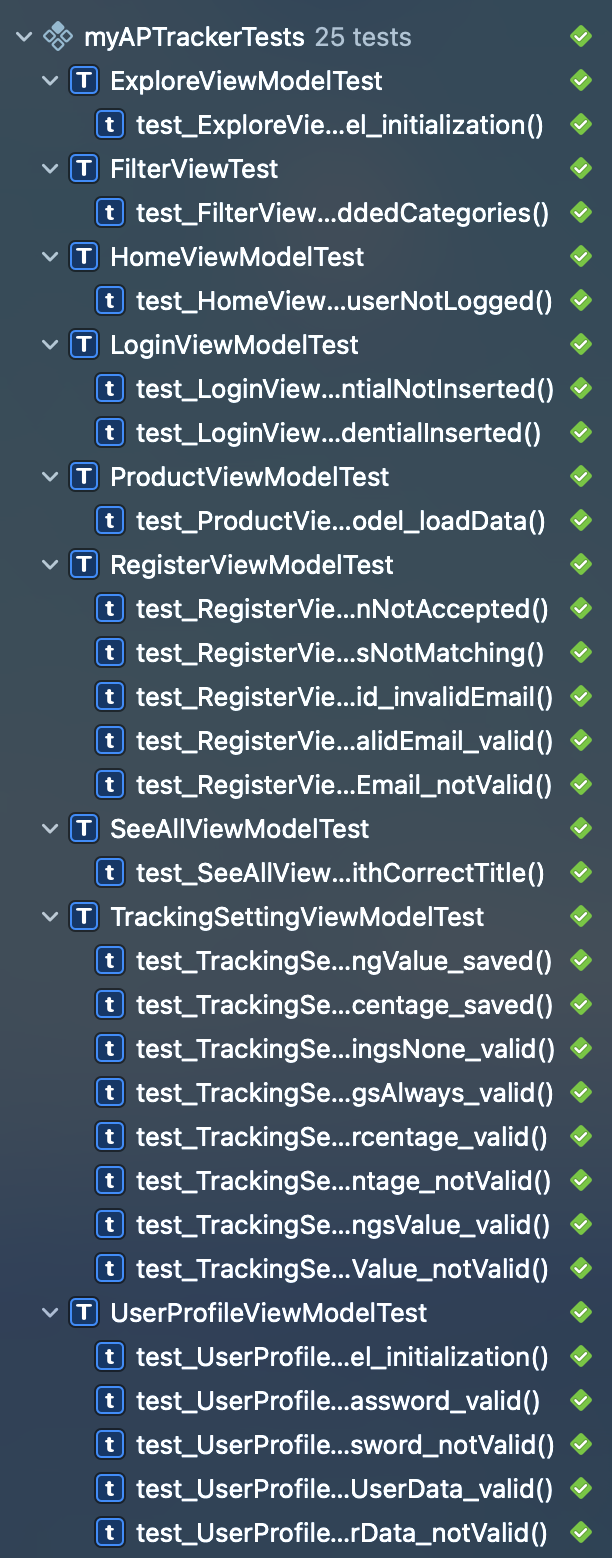
\includegraphics[scale=0.40]{images/testing/unit_testing.png}
        \caption{Unit testing}
        \label{fig:unit_testing}
\end{figure}
\FloatBarrier
In those test (figure: \ref{fig:unit_testing}) we have tested the logic of our application.
Some tests regard internal logic of the application, for instance if the values in the Shared Preferences were corrected or if after the initialization of a ViewModel the variables are correctly initialized.
While other test regard the testing of async calls to the API and the correct reception of the data, for the initialization phase and also for directly calls to the functions.

\newpage
\subsubsection{UI testing - iPhone}
\begin{figure}[h!]
        \centering
        \begin{subfigure}[b]{0.3\textwidth}
        \centering
            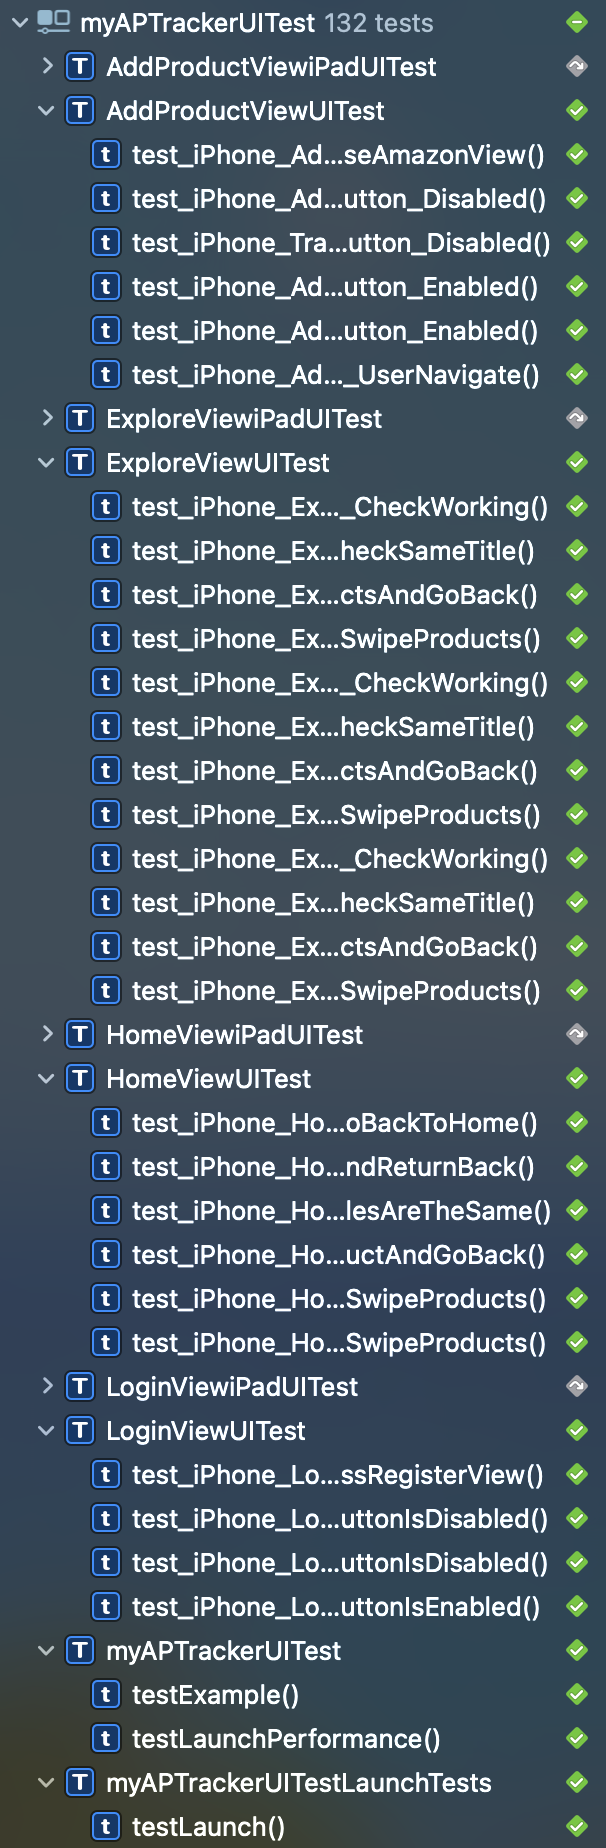
\includegraphics[width=\textwidth]{images/testing/ui_testing_iphone_1.png}
            \caption{iPhone 1}
            \label{fig:ui_testing_iphone_1}
        \end{subfigure}
        \begin{subfigure}[b]{0.3\textwidth}
            \centering
            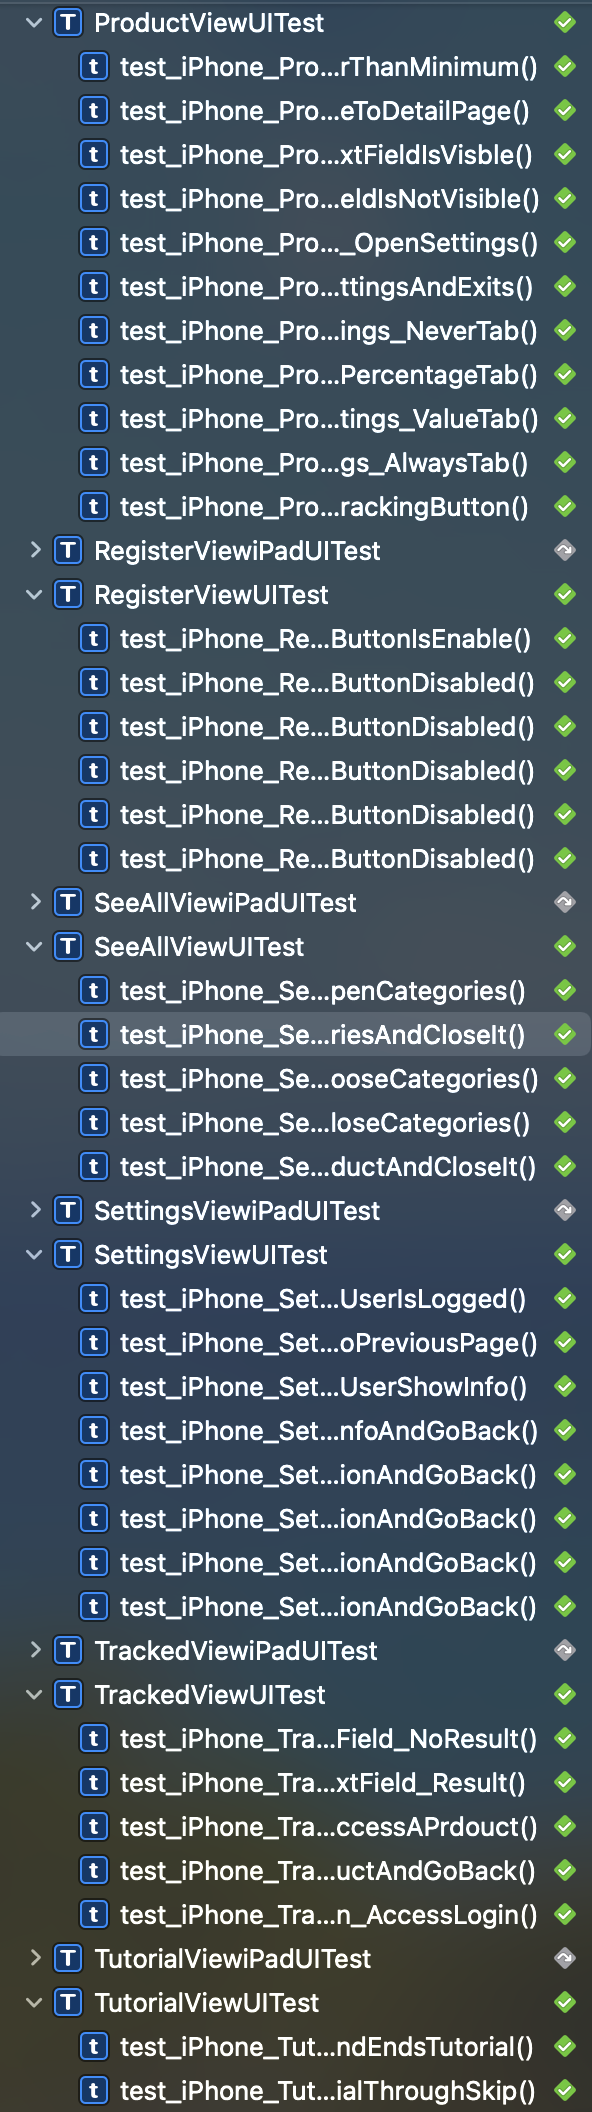
\includegraphics[width=\textwidth]{images/testing/ui_testing_iphone_2.png}
            \caption{iPhone 2}
            \label{fig:ui_testing_iphone_2}
        \end{subfigure}
         \caption{UI testing - iPhone}
        \label{fig:ui_testing_iphone}
\end{figure}
\FloatBarrier
In those test (figure: \ref{fig:ui_testing_iphone}) we have tested the UI of our application, only for the iPhone views, tests of iPad views are skipped.
We have tested the general working of our application from the point of view of an external user, therefore:
\begin{itemize}
    \item Navigation throughout the views.
    \item Presence of a precise view.
    \item Logic to enable buttons or disable it.
    \item Logic of different views (i.e. swipe to see more product, swipe to close a sheet, etc...).
    \item Navigation in the Amazon WebView.
\end{itemize}
To test the tutorialView, we have exploit the launchArguments() function of the XCTest framework, to pass as arguments a boolean to forcibly trigger (only for the test) the tutorial view to appear.
All the test have been adapted to manage a user logged in, but also if it is not logged in; furthermore, some tests have been done specifically for logged user and for non logged one (for instance we have tested the navigation in the WebView, where a logged user should see the "Track product" button, instead a non logged user should see the "Add product" button).
Finally, also the application flows (reported in section: "\nameref{subsection:application_flows}") have been tested.

\newpage
\subsubsection{UI testing - iPad}
\begin{figure}[h!]
        \centering
        \begin{subfigure}[b]{0.3\textwidth}
        \centering
            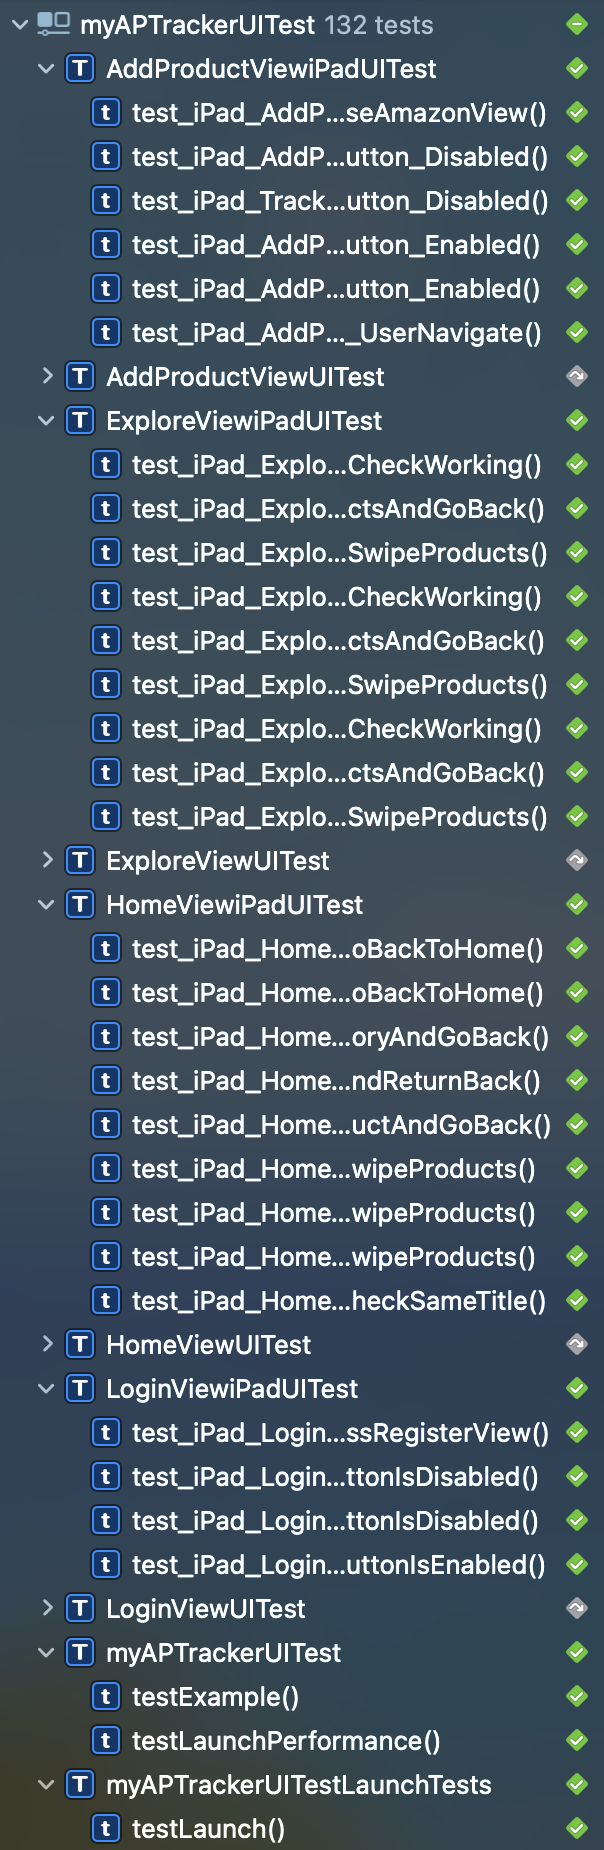
\includegraphics[width=\textwidth]{images/testing/ui_testing_ipad_1.png}
            \caption{iPad 1}
            \label{fig:ui_testing_ipad_1}
        \end{subfigure}
        \begin{subfigure}[b]{0.3\textwidth}
            \centering
            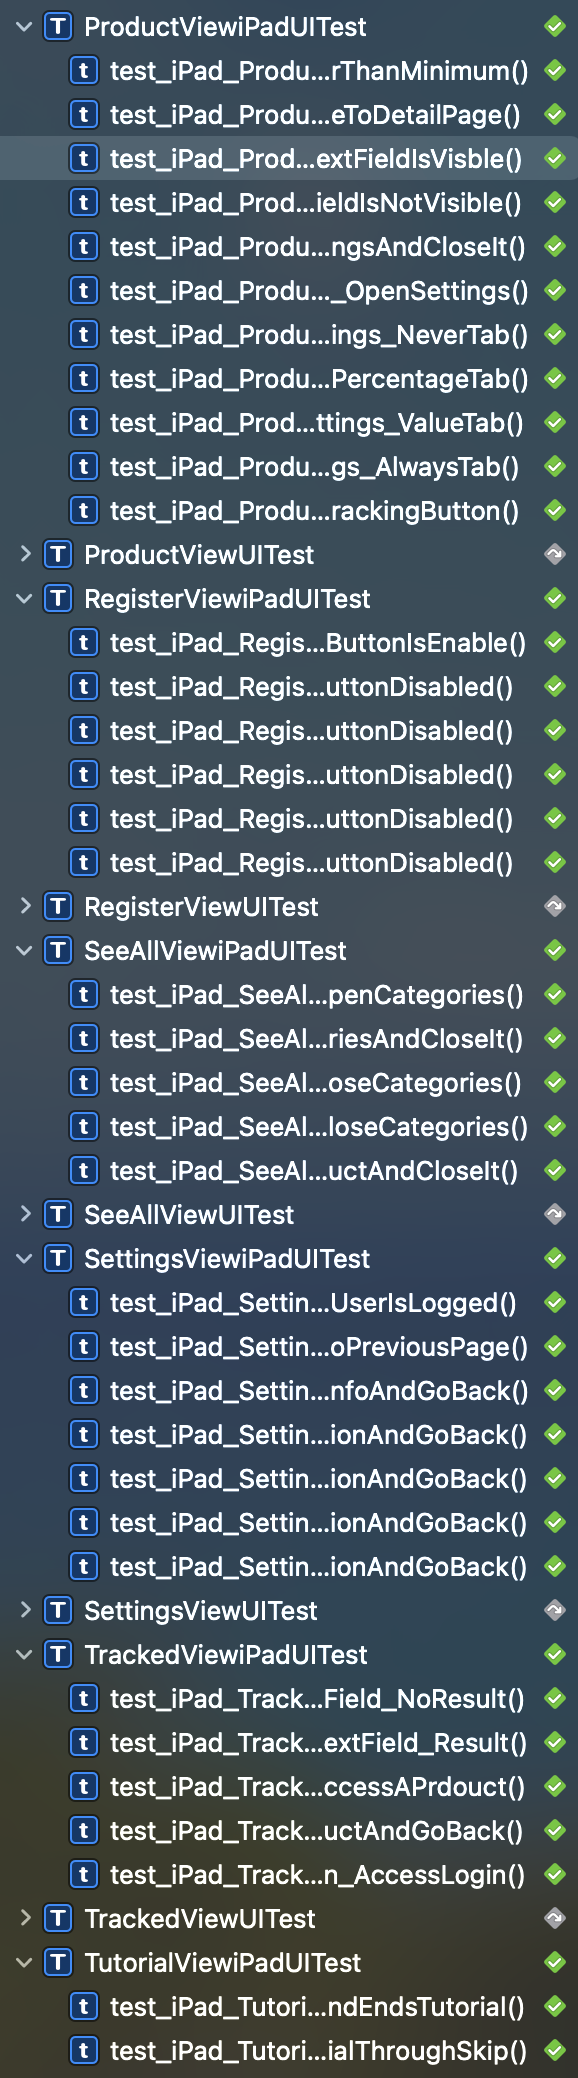
\includegraphics[width=\textwidth]{images/testing/ui_testing_ipad_2.png}
            \caption{iPad 2}
            \label{fig:ui_testing_ipad_2}
        \end{subfigure}
         \caption{UI testing - iPad}
        \label{fig:ui_testing_ipad}
\end{figure}
\FloatBarrier
In those test (figure: \ref{fig:ui_testing_ipad}) we have tested the UI of our application, only for the iPad views, tests of iPhone views are skipped.
We have tested the general working of our application from the point of view of an external user.
We have tested the same things as for iPhone but in this case the views are different, so different tests are needed.
Since the iPad supports both landscape and portrait orientation, the tests have been adapted to support both orientation.
A possibility it would have been to duplicate the tests modifying only the "setUpWithError" function, but it would have lead to a complete duplication of all the iPad tests.

\subsubsection{UI testing - Apple watch}
\begin{figure}[h!]
        \centering
        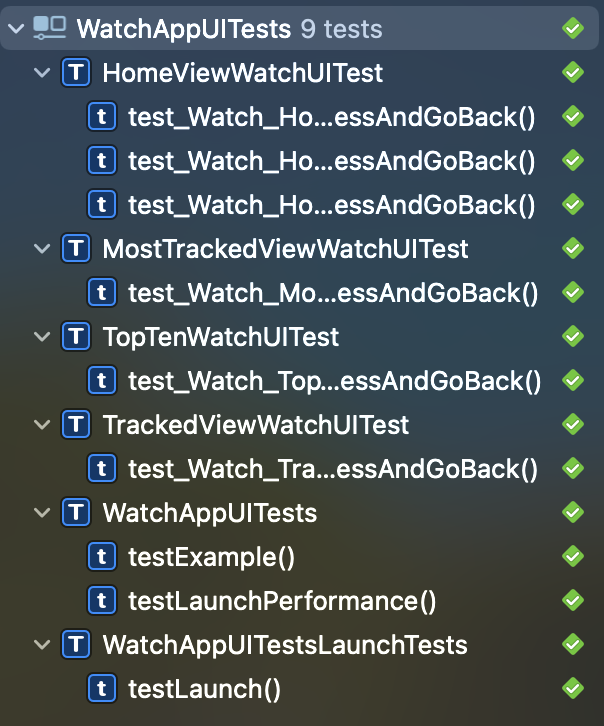
\includegraphics[scale=0.50]{images/testing/ui_testing_watch.png}
        \caption{UI testing Apple watch}
        \label{fig:ui_testing_watch}
\end{figure}
\FloatBarrier
In those test (figure: \ref{fig:ui_testing_watch}) we have tested the UI of our application, only for the Apple watch views.
We have tested the general working of our application from the point of view of an external user.

\subsubsection{TestFlight}
We have also created a test campaign through Apple TestFlight platform in order to have some people testing the application in a real scenario.\\
11 people tested the application functionalities alongside the implementation phase. In particular 11 beta have been released, the first 7 ones were released with the scope of testing new implemented functionalities, while the last 4 have been published in order to correct bugs and make improvements.\\
The last one is the current version (version 1.0 build 11) and it represents the pre-released one.

\subsection{Further implementations}
In this section will be presented some possible further implementations or improvements:

\begin{itemize}
    \item \textbf{Internationalization of Amazon website:} let the user access the Amazon website, corresponding to the user language.
    \item \textbf{Internationalization of the application:} this means not only the translation of the texts (in order that each user have access to the product available in its language), but the conversion of the currency and the correspondent price, based on the location of the user.
    \item \textbf{Improve user suggestion:} this means adding a ML layer in the back-end that suggests to the user some products in which they could be interested in.
    \item \textbf{Support more devices:} this can include a better and native support for MacOS since now the iPad application can be cross compiled keeping its UI.
\end{itemize}